\section{Detection Model Implementation}
\label{sec:ch3_detection}

This section describes the ROS~2 perception node used for brick detection and instance segmentation. The implementation is provided in \texttt{advanced\_detector\_node.py} and runs an Ultralytics YOLOv8s-seg model to produce per-brick bounding boxes, masks, orientations, and 3D poses in the camera frame.

\subsection{Dataset Preparation and Annotation}
The training dataset contains \textbf{9{,}525 images}. All labels were exported in \textbf{YOLOv8 format}, which is directly compatible with the Ultralytics training pipeline. Roboflow was used for data organization, annotation, and export, providing a consistent labeling interface, dataset versioning, and a reproducible export configuration.

\begin{figure}[H]
    \centering
    \begin{subfigure}[b]{0.32\textwidth}
        \centering
        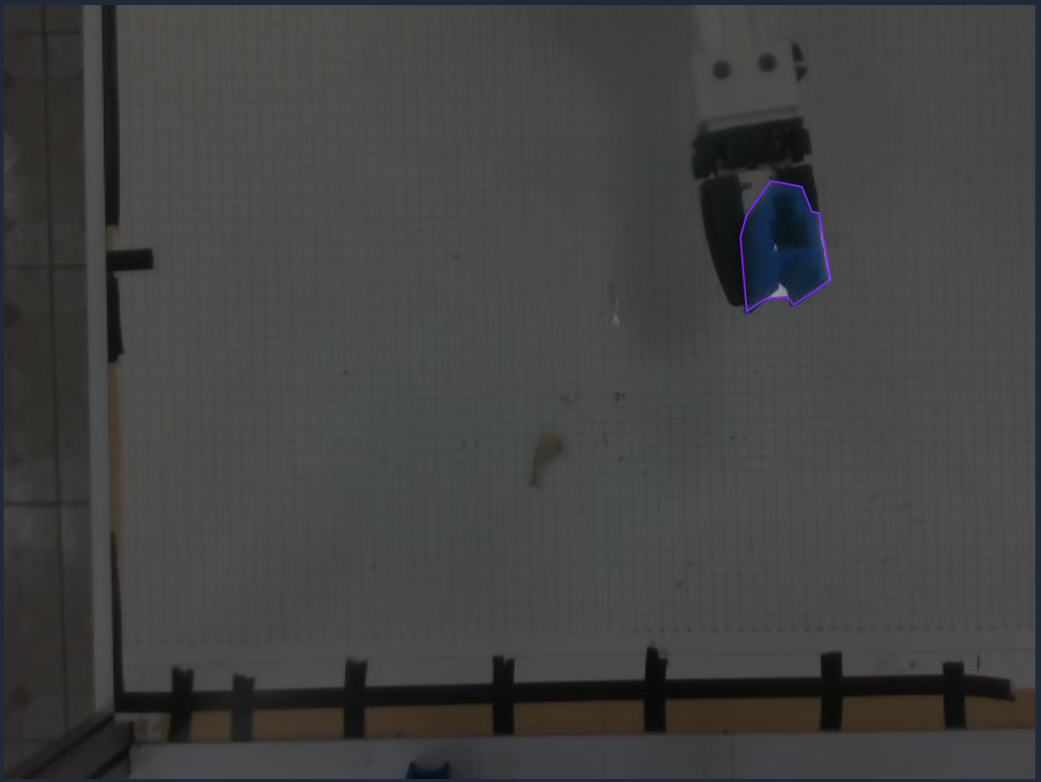
\includegraphics[width=\textwidth]{Figures/chapter3/Detection/I_shape.png}
        \caption{I-shape annotation sample.}
        \label{fig:anno_i_shape}
    \end{subfigure}
    \begin{subfigure}[b]{0.32\textwidth}
        \centering
        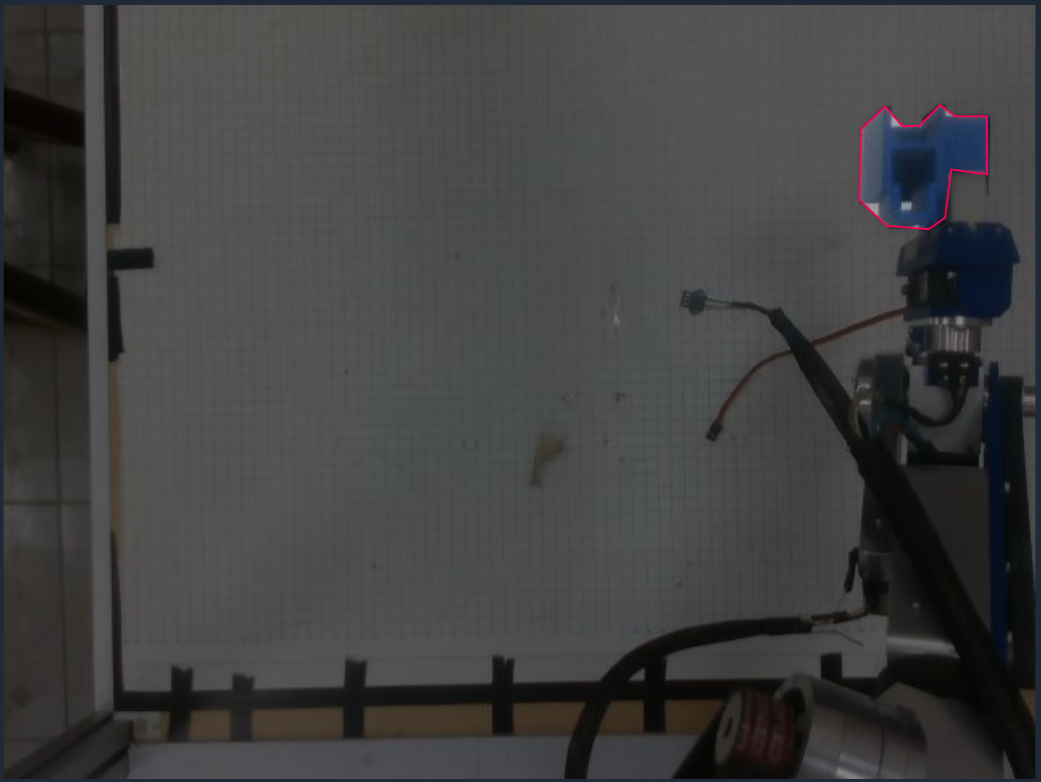
\includegraphics[width=\textwidth]{Figures/chapter3/Detection/L_shape.png}
        \caption{L-shape annotation sample.}
        \label{fig:anno_l_shape}
    \end{subfigure}
    \begin{subfigure}[b]{0.32\textwidth}
        \centering
        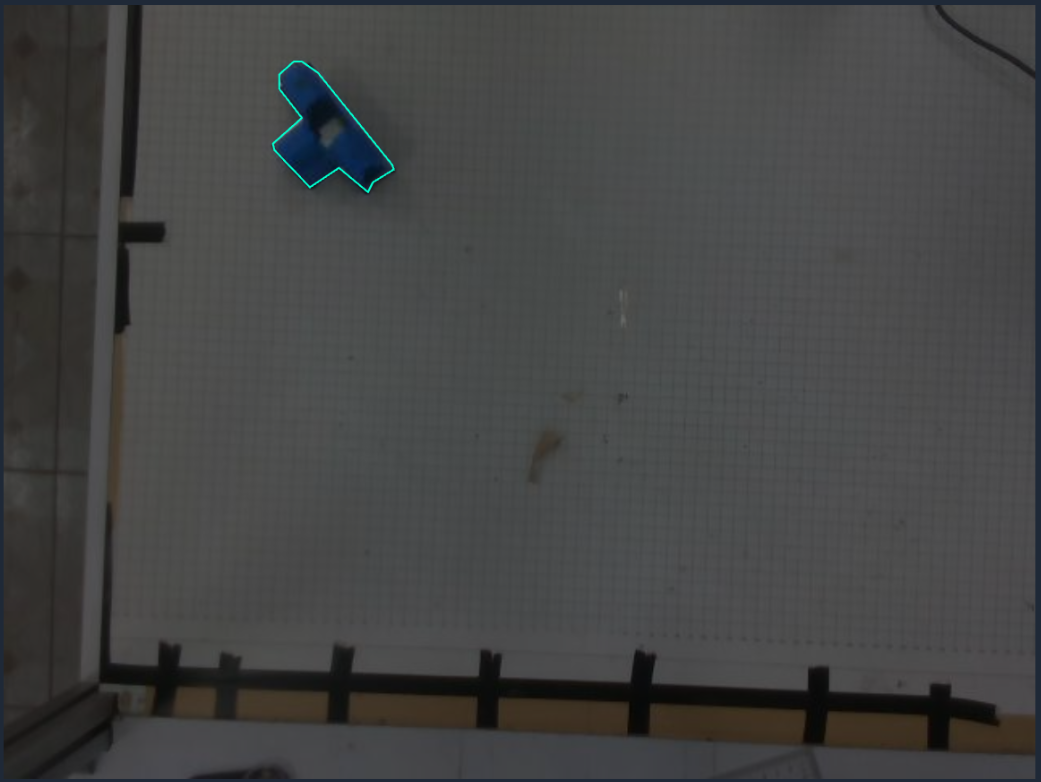
\includegraphics[width=\textwidth]{Figures/chapter3/Detection/T_shape.png}
        \caption{T-shape annotation sample.}
        \label{fig:anno_t_shape}
    \end{subfigure}
    \caption{Representative annotation samples for brick classes.}
    \label{fig:anno_samples}
\end{figure}

\subsection{Pre-processing and Augmentation}
To increase robustness to workspace variability, each source image was augmented to produce ten variants. The applied augmentations were:
\begin{itemize}
    \item 50\% probability of horizontal flip.
    \item Random rotation in the range $[-15^\circ, +15^\circ]$.
    \item Random brightness adjustment in the range $[-15\%, +15\%]$.
    \item Salt-and-pepper noise on 0.1\% of pixels.
\end{itemize}
These transformations improve generalization under changes in pose, illumination, and sensor noise while preserving the geometric structure of the bricks.

\begin{figure}[H]
    \centering
    \begin{subfigure}[t]{0.32\textwidth}
        \centering
        \vspace{0pt}
        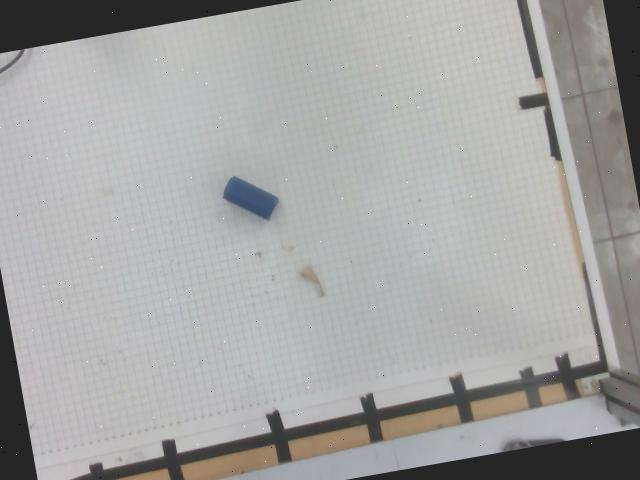
\includegraphics[height=3.2cm, keepaspectratio]{Figures/chapter3/Detection/augmentation/rotation.jpg}
        \caption{Rotation augmentation.}
        \label{fig:aug_rotation}
    \end{subfigure}
    \begin{subfigure}[t]{0.32\textwidth}
        \centering
        \vspace{0pt}
        
\includegraphics[height=3.2cm, keepaspectratio]{Figures/chapter3/Detection/augmentation/brightness.png}
        \caption{Brightness augmentation.}
        \label{fig:aug_brightness}
    \end{subfigure}
    \begin{subfigure}[t]{0.32\textwidth}
        \centering
        \vspace{0pt}
        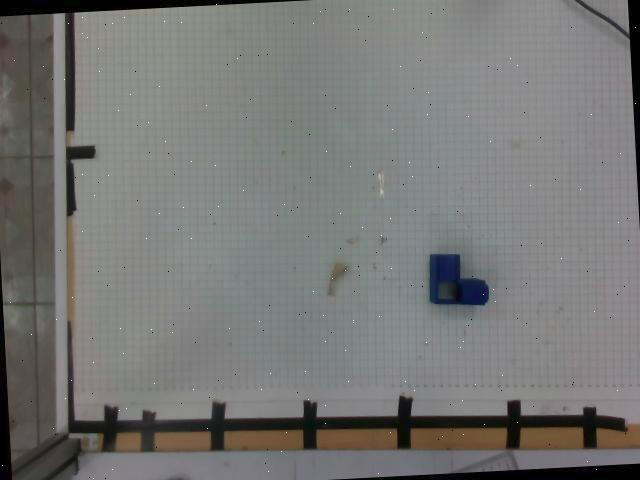
\includegraphics[height=3.2cm, keepaspectratio]{Figures/chapter3/Detection/augmentation/salt_and_paper_noise.png}
        \caption{Salt-and-pepper noise augmentation.}
        \label{fig:aug_noise}
    \end{subfigure}
    \caption{Examples of data augmentation applied to the brick dataset.}
    \label{fig:augmentation_examples}
\end{figure}

\subsection{Training Procedure (YOLOv8s-seg)}
Training was performed using the Ultralytics YOLOv8 segmentation pipeline with the exported YOLOv8-format dataset. The model selected for deployment is \textbf{YOLOv8s-seg}, which provides a strong accuracy--speed trade-off for real-time robotic perception. The training process follows the standard YOLOv8 workflow: dataset loading, multi-scale feature learning, joint optimization of detection and segmentation objectives, and evaluation on held-out data.

\subsection{Node Structure and Parameters}
The node is implemented as \texttt{YoloV8Detector}, a standard \texttt{rclpy} node. Key runtime parameters are:
\begin{itemize}
    \item \texttt{image\_topic}: input RGB image topic (default: \texttt{/camera/camera/color/image\_raw}).
    \item \texttt{camera\_info\_topic}: camera calibration topic (default: \texttt{/camera/camera/color/camera\_info}).
    \item \texttt{pixels\_per\_cm}: pixel-to-centimeter scale for grid projection (default: 8.0).
    \item \texttt{camera\_frame}: frame ID assigned to outputs (default: \texttt{camera\_color\_optical\_frame}).
\end{itemize}

\subsection{Subscribed and Published Interfaces}
The node subscribes to:
\begin{itemize}
    \item \texttt{Image} for RGB frames.
    \item \texttt{CameraInfo} for intrinsics $\{f_x, f_y, c_x, c_y\}$.
\end{itemize}

It publishes:
\begin{itemize}
    \item \texttt{/yolo/annotated\_image} (\texttt{Image}) containing color-coded overlays and axes.
    \item \texttt{/yolo/detections} (\texttt{Detection2DArray}) with per-object 2D boxes and scores.
    \item \texttt{/detected\_bricks} (\texttt{BricksArray}) with 3D pose, ID, class, and workspace side.
    \item \texttt{/yolo/markers} (\texttt{MarkerArray}) for RViz visualization of brick poses.
\end{itemize}

\subsection{Inference and Tracking Pipeline}
For each incoming frame:
\begin{enumerate}
    \item The RGB message is converted to an OpenCV \texttt{bgr8} image using \texttt{CvBridge}.
    \item YOLOv8s-seg is executed with \texttt{retina\_masks=True}, yielding bounding boxes and (optionally) polygon masks.
    \item Each detection is represented by center $(c_x, c_y)$, box corners $(x_1, y_1, x_2, y_2)$, class label, confidence, and orientation (computed from the mask when available).
    \item Detections are passed to a \texttt{BrickTracker} for ID assignment and temporal stability using a distance-based association (\texttt{distance\_threshold=60}) and \texttt{max\_disappeared=300}.
\end{enumerate}

\subsection{Index Tracking and ID Consistency}
To maintain consistent brick indices across frames, we use a lightweight centroid-based tracker (\texttt{BrickTracker}). Each detection is represented by its 2D center $(c_x, c_y)$, and detections are matched frame-to-frame by minimizing the Euclidean distance between current centers and previously tracked centers. If the closest match is within a configurable threshold (\texttt{distance\_threshold=60}), the detection inherits the existing ID; otherwise, a new ID is assigned.

The tracker also handles temporary occlusions and missed detections using a \texttt{max\_disappeared=300} counter. If an object is not observed for a limited number of frames, its track is preserved, allowing the ID to remain stable when the object reappears. Once the disappearance counter exceeds the threshold, the track is removed to prevent stale IDs from accumulating.

This strategy provides:
\begin{itemize}
    \item \textbf{Stable indexing} for downstream modules that rely on persistent brick IDs.
    \item \textbf{Robustness to brief occlusions} and detector dropouts.
    \item \textbf{Low computational cost}, suitable for real-time operation.
\end{itemize}

\subsection{Orientation Estimation using Principal Component Analysis (PCA)}
\textbf{PCA (Principal Component Analysis):} We use PCA to get the orientation of the brick (yaw) as our detection model (YOLO) doesn’t output the orientation of the brick, only the bounding box; we use the PCA function in the OpenCV Python library.

While the YOLOv8 model is highly effective at object detection and classification, it is inherently limited to outputting axis-aligned bounding boxes (AABB). These bounding boxes provide the object's class and centroid coordinates $(u, v)$ but fail to provide the rotational orientation (yaw) of the plastic bricks. For a collaborative pick-and-place task, the robotic gripper must align its jaws with the brick’s principal axis to ensure a stable grasp. To bridge this gap, we utilize Principal Component Analysis (PCA) via the OpenCV library.

\begin{figure}[H]
    \centering
    
\includegraphics[width=0.9\textwidth]{Figures/chapter3/Detection/pca_vectors.jpeg}
    \caption{PCA principal axes overlaid on brick contours.}
    \label{fig:pca_vectors}
\end{figure}

\subsubsection{Theoretical Background of PCA}
Principal Component Analysis is a statistical technique used primarily for dimensionality reduction, but in the context of computer vision, it is utilized to identify the primary axes of geometric spread within a set of data points. By analyzing the covariance matrix of the brick's contour points, PCA extracts the eigenvectors and eigenvalues:
\begin{itemize}
    \item \textbf{Eigenvectors} represent the directions of the data's spread.
    \item \textbf{Eigenvalues} represent the magnitude of the spread along those directions.
\end{itemize}
For a rectangular plastic brick, the first principal component (the eigenvector associated with the largest eigenvalue) aligns with the object's length (major axis), while the second principal component aligns with its width (minor axis).

\subsubsection{Implementation Pipeline}
The orientation extraction process follows these steps:
\begin{enumerate}
    \item \textbf{Region of Interest (ROI) Extraction:} The bounding box coordinates from the YOLO inference are used to crop the specific brick from the main video frame.
    \item \textbf{Segmentation:} Binary thresholding is applied to the cropped ROI to isolate the brick’s pixels from the background, generating a binary mask.
    \item \textbf{Contour Extraction:} The boundary points of the brick are extracted from the binary mask. These $(x, y)$ coordinates form the dataset for the analysis.
    \item \textbf{PCA Computation:} Using the OpenCV function \texttt{cv2.PCACompute2}, we calculate the mean and eigenvectors of the contour points.
    \item \textbf{Orientation Calculation:} The orientation angle $\theta$ is derived from the primary eigenvector components $(v_x, v_y)$ using:
    $$
    \theta = \arctan2(v_y, v_x)
    $$
\end{enumerate}
This angle is then converted from radians to degrees and passed to the grasping planner to adjust the robot's end-effector yaw ($\psi$).

\subsubsection{Intuitive Explanation}
PCA finds the dominant direction in a cloud of points. For an elongated object such as a brick, the longest spread corresponds to its length, and the direction of that spread gives the orientation. We compute PCA on the contour pixels; the first principal component points along the brick's major axis, and its angle indicates whether the brick is vertical, horizontal, or tilted.

\subsubsection{Limitations of Bounding Box Representation}
YOLO outputs boxes that are parallel to the image axes. If a brick is rotated by $45^\circ$, the axis-aligned box does not capture that tilt. PCA, however, uses the actual shape inside the box and therefore recovers the true orientation.

\subsection{Workspace Partition and Grid Region}
The image is partitioned into two robot workspaces using a horizontal split at $0.42H$. A square grid region of size 24~cm is projected into pixel space using \texttt{pixels\_per\_cm} and centered at an offset $(W/2 + 56, \; 0.42H)$. Each brick is assigned to one of three regions:
\begin{itemize}
    \item \textbf{GRID}: inside the grid square.
    \item \textbf{ABB}: above the split line.
    \item \textbf{AR4}: below the split line.
\end{itemize}
These labels are stored in the \texttt{Brick.side} field and are also used for color-coded overlays.

\subsection{3D Pose Estimation in Camera Frame}
If camera intrinsics are available, the node back-projects the 2D center into 3D using the depth $Z$ obtained from the camera:
$$
X = \frac{(c_x - c_x^0) \, Z}{f_x}, \quad
Y = \frac{(c_y - c_y^0) \, Z}{f_y}
$$
The orientation is converted to a quaternion about the $Z$ axis and stored in \texttt{Brick.pose.orientation}. If intrinsics are missing, a fallback pixel-offset representation is used for $X$ and $Y$.
